
\subsection{Work Breakdown Structure}

The team is categorized into different groups of responsibilities with dedicated leaders who will report to and coordinate with the Project Manager. Leadership may be organized on a rotational basis should the need arise. The formation of these divisions constitute a work breakdown structure in which is illustrated in Figure \ref{fig:work-breakdown-structure}.


The interaction between the divisions will be refined over the course of project implementation to acknowledge the interdisciplinary nature of the experiment around a Payload / Platform scheme.

The Management is composed of a Project Manager and a Deputy Project Manager, both acting as Systems Engineer and managing overall implementation of the project. The Project Manager is responsible for establishing and overseeing product development cycle; coordinating between different teams, project stakeholders, and documentation efforts; outreach and public relations; Fundraising; monitoring and reporting; system integration; and quality assurance. The Deputy Project Manager assists the Project Manager in all management duties in a manner that ensures replaceability when necessary.

The Scientific Division is responsible for defining experiment parameters; data analysis; interpreting and documenting measurements; researching previous CAC experiments for comparative analysis purposes; evaluating the reliability of the proposed AAC sampling system; conducting measurements of collected samples; documenting and publishing findings; defining experiment parameters; contacting researchers or institutions working on similar projects; exploring potential partnership with researchers and institutions; documenting and publishing findings.

The Mechanical Division is responsible for designing or redesigning cost-effective mechanical devices using analysis and computer-aided design; producing details of specifications and outline designs; overseeing the manufacturing process for the devices; identifying material and component suppliers; developing and testing prototypes of designed devices; analyzing test results and changing the design as needed; and integrating and assembling final design.

The Electrical Division is responsible for designing and implementing cost-effective circuitry using analysis and computer-aided design; producing details of specifications and outline designs; developing, testing, and evaluating theoretical designs; identifying material as well as component suppliers; reviewing and testing proposed designs; recommending modifications following prototype test results; and assembling designed circuitry.

The Software Division is responsible for gathering software requirements; formalizing software specifications; drafting architecture design; leading software implementation efforts; leading quality assurance and testing efforts; enforcing software testing best practices such as continuous integration testing and regression testing; reviewing requirements and specifications in order to foresee potential issues; providing input for functional requirements; advising on design; formalizing test cases; tracking defects and ensuring their resolution; facilitating code review sessions; and supporting software implementation efforts.

The Thermal Division is responsible for ensuring thermal regulation of the payload as per operational requirements of all experiment components; evaluating designs against thermal simulation and propose improvements; managing against mechanical design and electrical power limitations towards providing passive and active thermal control systems.

\begin{landscape}
\begin{figure}[p]
    \begin{align*}
        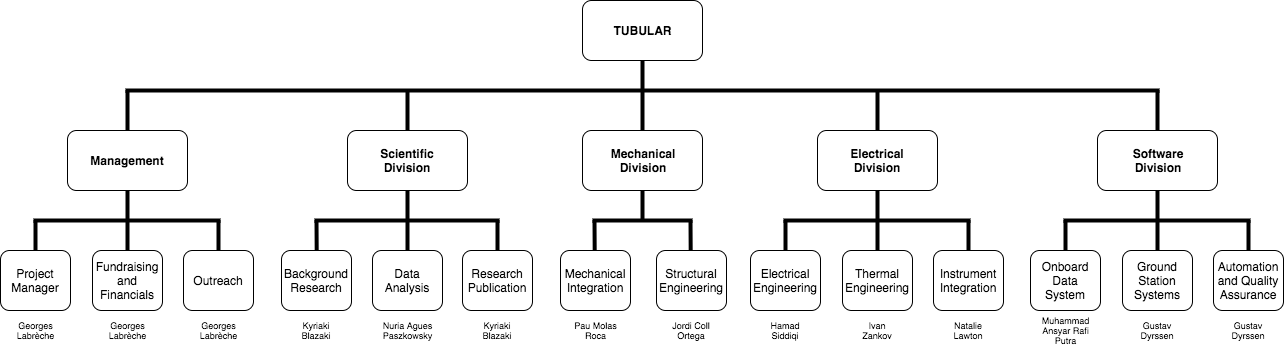
\includegraphics[width=24cm]{3-project-planning/img/work-breakdown-structure.png}
    \end{align*}
    \caption{Work Breakdown Structure}\label{fig:work-breakdown-structure}
\end{figure}
\end{landscape}